\documentclass[a4paper, 12pt]{article}

\usepackage[T1]{fontenc}
\usepackage[utf8]{inputenc}
\usepackage[english]{babel}  % ngerman for German
\usepackage{lmodern}  % nicer font
\usepackage{geometry}
\geometry{%
	left   = 2.5cm,
	right  = 2.5cm,
	top    = 3cm,
	bottom = 3cm
}

\usepackage{textcomp}
\usepackage{gensymb}
\usepackage{amsmath,amssymb,amsfonts}
\usepackage{nicefrac}  % nicer inline fractions
\usepackage{tensor}  % allows fancy indices
\usepackage{siunitx}  % easy handling of value + unit (e.g. \SI{10}{\pF})
% \sisetup{}  % configure siunitx (e.g. locale = DE)
\sisetup{output-complex-root=\ensuremath{\mathrm{j}}, complex-root-position = before-number} % configures SI format 10 + j5 for complex numbers (instead of 10 + 5i)

\usepackage{listings}  % code listings
\usepackage{verbatim}  % inline code (\verb||)
\usepackage{enumerate}
\usepackage[shortlabels]{enumitem}  % simple format for enumerations (e.g. 
\usepackage{booktabs}  % nicer tables (e.g. \toprule)
\usepackage{subcaption}  % captions for subplots
\usepackage[european, siunitx, RPvoltages]{circuitikz}  % draw circuit diagrams

\setlist[itemize]{label=\rule[0.5ex]{0.6ex}{0.6ex}} % black squares for itemize

\usepackage{pstool}  %% Tex fonts in EPS files
\usepackage{graphicx}
\graphicspath{{./figures/}}

\setlength {\marginparwidth }{2cm}  % fixes issue with todonotes
\usepackage{todonotes}
\usepackage{etoolbox} % Needed for AtBeginEnvironment command (appendix handling)
\usepackage{appendix} % Appendices environment

\usepackage{csquotes} % removes biber warning
\usepackage[  % ieee style citations (e.g. [1])
	backend     = biber,
	maxbibnames = 99,
	autocite    = footnote,
	style	    = ieee,
	citestyle   = numeric-comp,
	doi=false, isbn=false
]{biblatex}
\addbibresource{bibliography/bibliography.bib}

\usepackage[nobiblatex]{xurl}  % line breaks in URLs
% last imports
\usepackage[bookmarksopen,colorlinks,citecolor=black,linkcolor=black, urlcolor = black]{hyperref}

% after hyperref! 
\usepackage[noabbrev, nameinlink]{cleveref} 
% e.g. \cref{label} or \Cref(label) for capital letter
% configure cleveref not to use brackets around equation references
\creflabelformat{equation}{#2\textup{#1}#3} % Equation references without parentheses
\AtBeginEnvironment{appendices}{\crefalias{section}{appendix}} % Appendix referencing (for cref "Appendix A" instead of "Section A")


% add missing hyphenations
\hyphenation{im-ple-men-ta-tions}

\title{384.178 SoC Design Lab\\
	   Integration of an Encryption Accelerator
	   into an Open-Source Low-Power Microcontroller}
\author{
  Severin Jäger, 01613004
}
\date{\today}


\begin{document}

\maketitle
\tableofcontents
\pagebreak

\section{Introduction} \label{sec:intro}

Extreme edge devices are increasingly facing signal processing workloads. Sensor signals are frequently processed directly in the sensor node before being transmitted for further analysis. Examples include simple machine learning algorithms detecting relevant sequences or events in a sensor signal. However, such edge devices are usually battery powered and designed for a long lifetime, thus the energy consumption is highly constrained. So, all applications have to be designed with energy efficiency in mind. This is also a main factor when partitioning between hardware and software.

One major academic project focussing on energy-efficient processor and system design is the PULP platform~\cite{pulp} by ETH Zurich and University of Bologna. Over the last years, the developed several processor cores as well as peripherals and full systems on chips (SoCs). Utilising the open source instruction set architecture RISC-V, the RTL code of the IP cores developed within this project is available publicly with a permissive license.

In certain applications including biomedical devices, video surveillance, or home automation, traditional requirements are complemented by a need for confidentiality. Thus, standard cryptographic algorithms have to be executed on the hardware. Unfortunately, processing these algorithms in software is relatively complex and consumes significant memory, time, and thus energy. These issues might however be alleviated by offloading the computation to a dedicated cryptographic accelerator. The scope of this project is integrating and open-source hardware accelerator into the PULPissimo SoC~\cite{Schiavone2018} and comparing it to a pure software solution.

This report is structured as follows. Firstly, \Cref{sec:background} discussed the relevant background including the PULPissimo SoC and AES hardware. Then, \Cref{sec:implementation} elaborates on the work conducted during this project. \Cref{sec:results} outlines the key results before \Cref{sec:summary} concludes this report. 

\section{Background} \label{sec:background}

\subsection{PULPissimo}

PULPissimo is a microcontroller and as such one of the smallest platforms within the PULP ecosystem. It comes with a single RISC-V core, memory, a DMA controller and a full set of peripherals connected to a peripheral bus. Furthermore, it allows the convenient integration of a so-called hardware processing engine (HWPE) which directly operates on the memory. The SoC architecture is depicted in \cref{pulpissimo-arch}.

The design is mainly targeting ASIC technology and focussed on maximum energy efficiency. In a \SI{22}{nm} FDX technology, an energy efficiency of \SI{433}{MOPS/mW} has been shown~\cite{Schiavone2018}. The full System Verilog RTL code is available on GitHub~\cite{pulpissimo}.

\begin{figure}
	\centering
	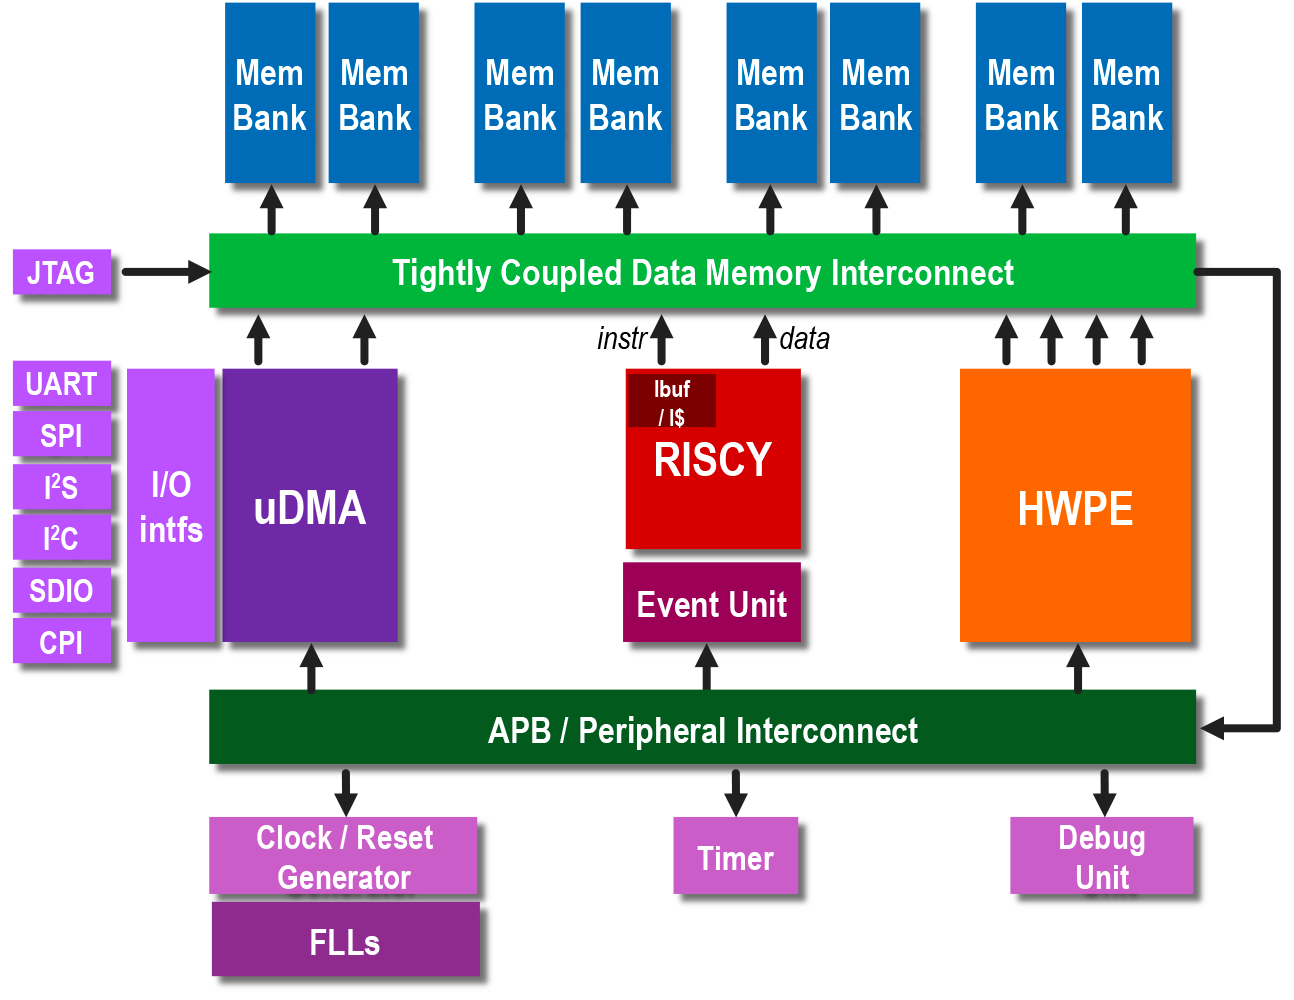
\includegraphics[width=0.65\textwidth]{pulpissimo_arch.png}
	\label{pulpissimo-arch}
	\caption{Architecture of the PULPissimo SoC \cite{pulpissimo}}
\end{figure}

\subsubsection*{Hardware Processing Engine (HWPE)}

The PULP hardware processing engine is a quite unique hardware accelerator. As depicted in \Cref{hwpe-arch}, it consists of a data interface, a control interface and the data path. In contrast to most accelerators in literature it neither uses a dedicated accelerator interface in the CPU nor direct memory access (DMA) to get the data to process. Instead, it shares the so-called tightly coupled memory (which somehow corresponds to an L2 cache) with the processor core. The control interface is connected to the peripheral bus and is thus seen as a memory-mapped peripheral by the CPU. It provides configuration registers which can be written by the processor.

A typical HWPE operation works as follows. Firstly, the relevant data has to be in the shared memory. Then, the CPU sets all relevant configuration data (e.g. pointers of source and destination in shared memory, HWPE configuration) in the HWPE via the control interface. Once an HWPE operation is started, it operates fully autonomous and the CPU can perform other computations. After completion, the HWPE trigger and event which can be polled in the CPU or raise an interrupt. The event indicates that the output data is written to the shared memory.

HWPEs are not limited to PULPissimo, but can also be integrated into more powerful SoCs within the PULP project including multicore systems and HPC clusters. Thus, the effort of designing an HWPE can be reused easily. Furthermore, a template HWPE implementing a multiply-accumulate (MAC) engine is available~\cite{hwpe-mac}. This template features a relatively simple data path, but a powerful control interface including a microcode processor and a finite state machine as well as three 32 bit inputs and one 32 bit output. The template is intended as starting point for new HWPEs and alleviates the burden of the developer to write a device driver and to handle the memory access.

\begin{figure}
	\centering
	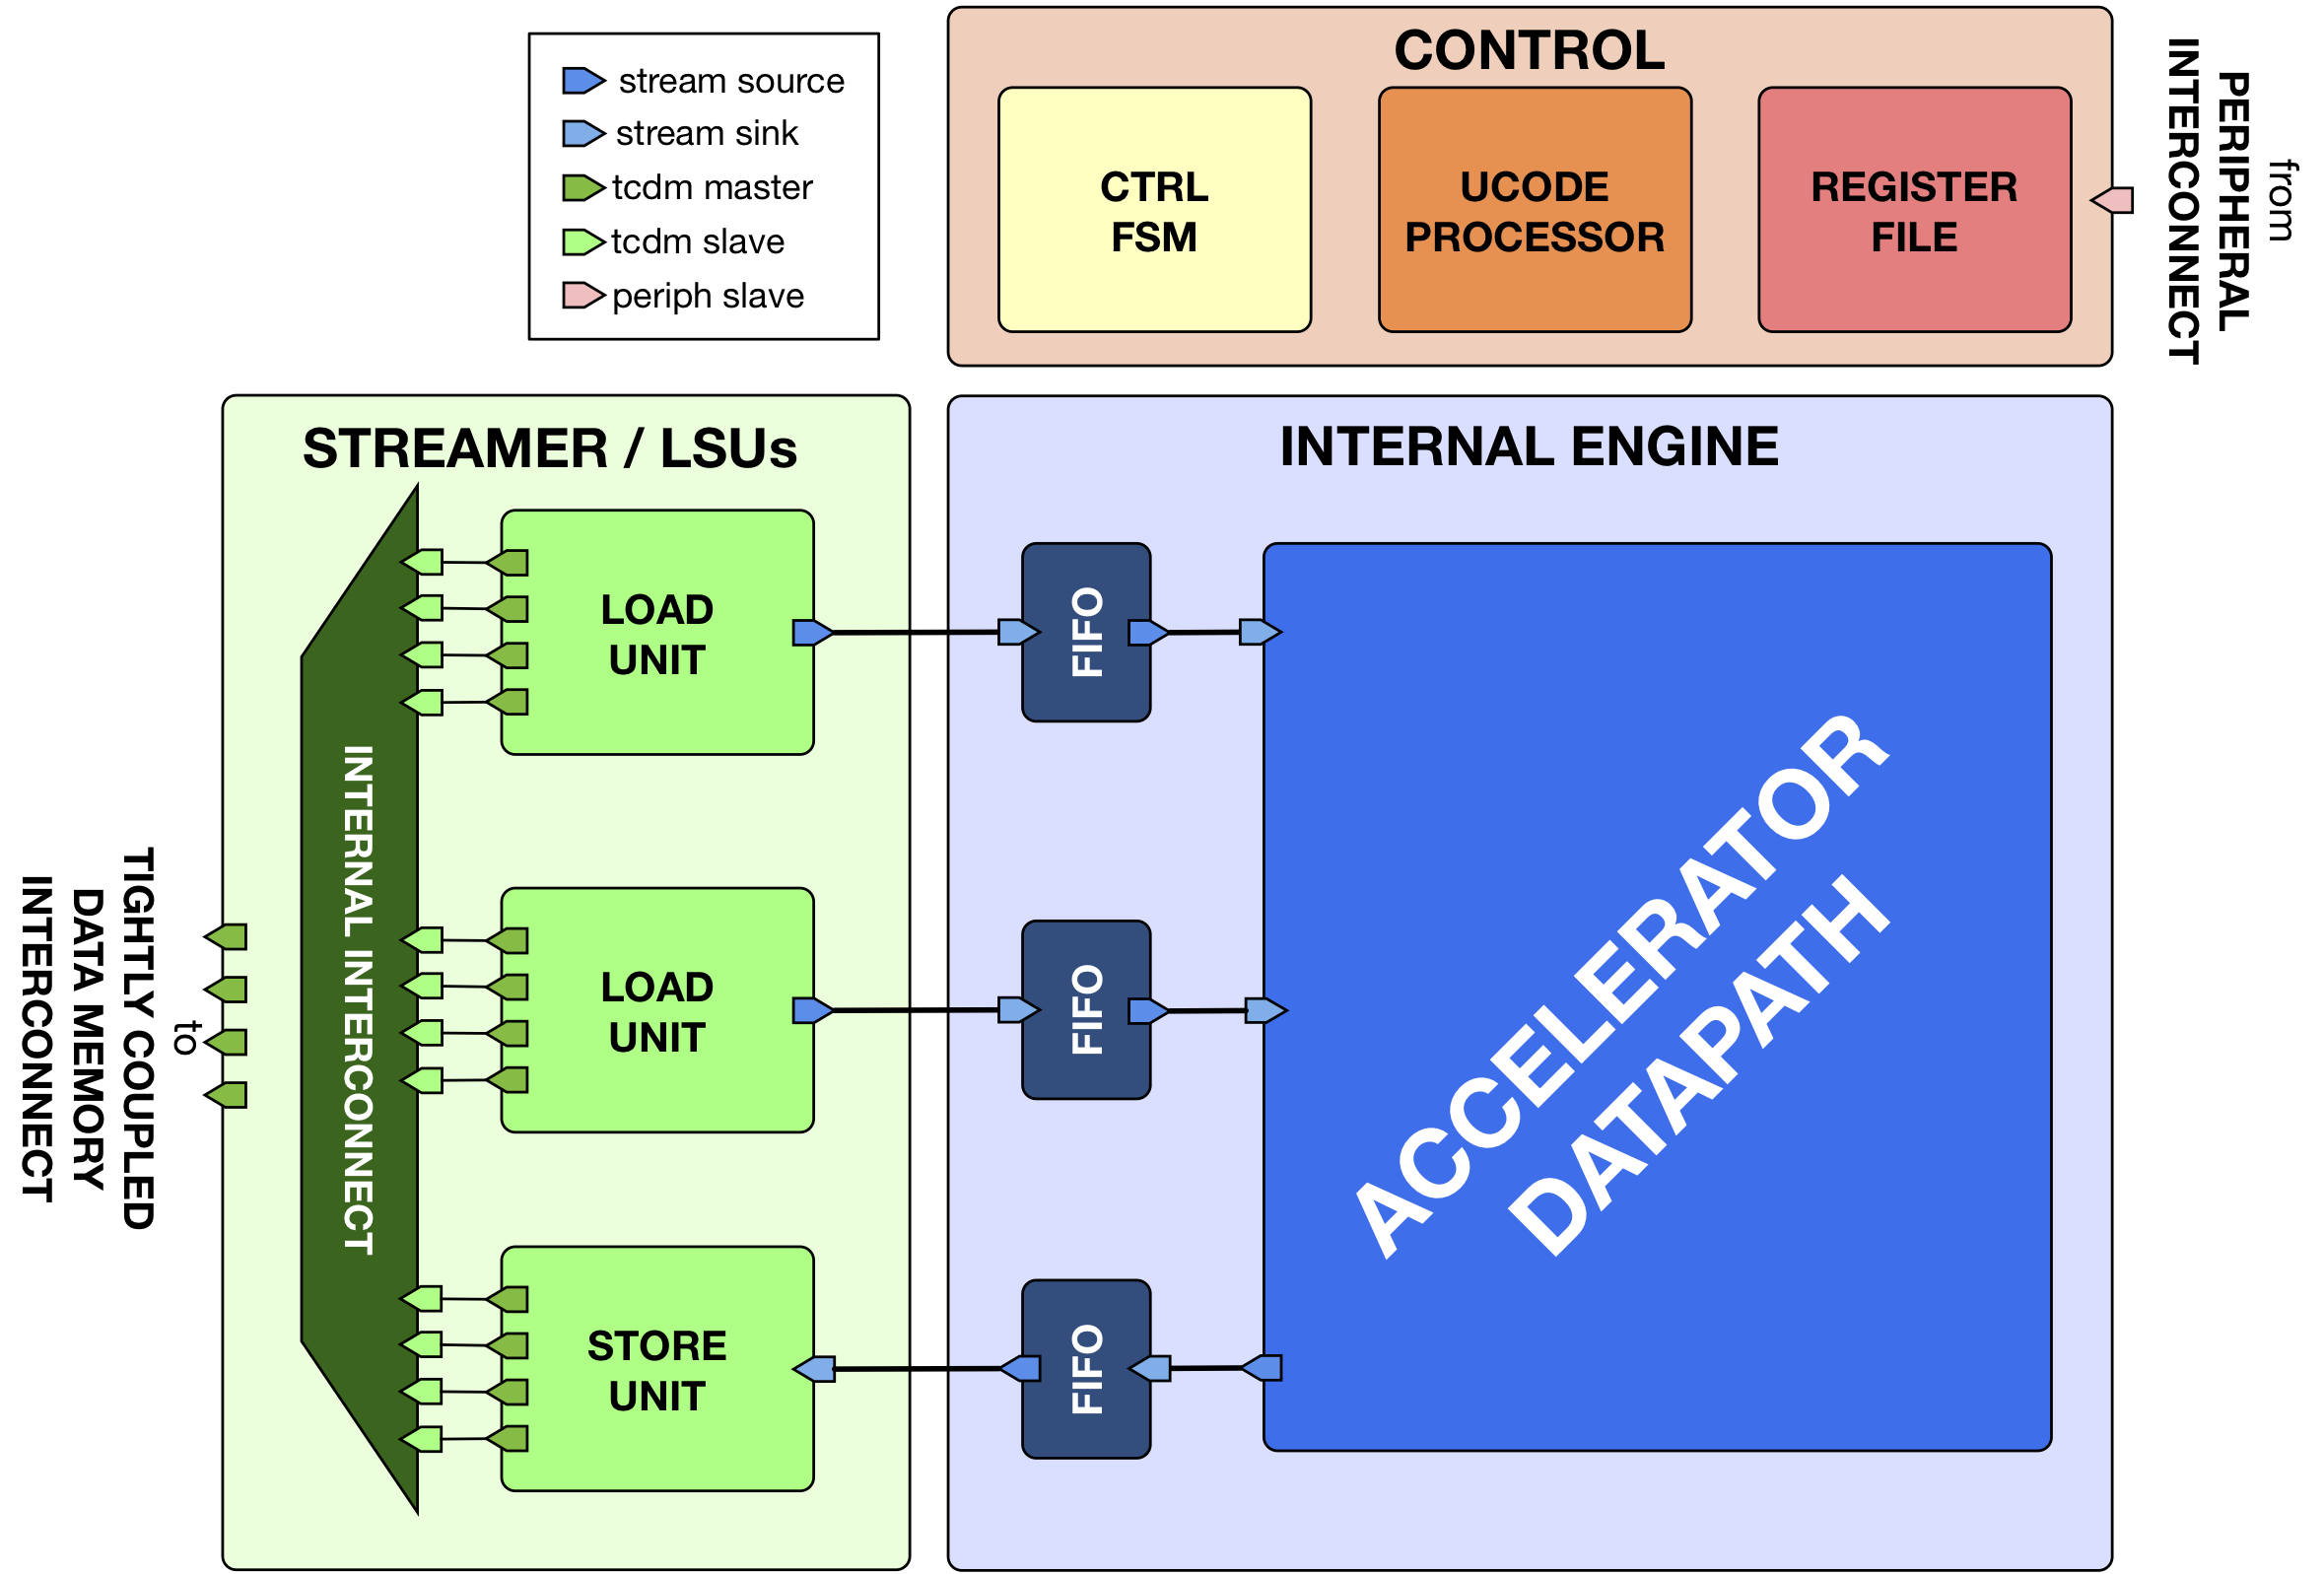
\includegraphics[width=0.65\textwidth]{hwpe.png}
	\label{hwpe-arch}
	\caption{Architecture of a PULP Hardware Processing Engine \cite{hwpe}}
\end{figure}

\subsection{AES Hardware}

The advanced encryption standard (AES) defines a set of block cipher algorithms which are also known under their original name Rijndael. It works on 128 bit words and uses either 128, 192, or 256 bit long keys. The algorithm was designed for straightforward hardware implementation and is one of the most used block ciphers.

Thus, several hardware implementation of the AES algorithms are available. As this project uses open-source System Verilog RTL code, only open-source Verilog implementations were considered. \Cref{tab:aes_cores} compares the three IP cores considered. An edge device requires only encryption capabilities to transfer sensor data in a secure way. Also due to size and energy limitations, only AES with 128 bit keys was considered.

\begin{table}[h]
    \centering
    \begin{tabular}{c|c c c}
        \toprule
        Core &  \verb|tiny_aes|~\cite{tiny-aes} & \verb|aes_128|~\cite{aes-128} & \verb|secworks_aes|~\cite{secworks-aes}  \\
        \midrule
        Cycles/Op &  1 & 12 & 4\\
        Latency (cylces) & 21 & 12 & 14\\
        LUTs & 4588 & 487 & 3327 \\
        Registers & 4474 & 402 & 2990 \\
        BRAM Tiles & 68 & 5 & 0 \\
        Max. Frequency [MHz] & 375.9 & 180.5 & 124.8 \\
        Decryption & no & no  & yes \\
        256 bit keys & no & no & yes\\
        \bottomrule
    \end{tabular}
	\label{tab:aes_cores}
	\caption{Comparison of selected open-source AES IP cores. Resource consumption and clock frequency were obtained with Vivado 2020.2 synthesising for a Nexys4DDR evaluation board.}
\end{table}

Clearly, the \verb|tiny_aes| core provides the best performance. It is fully pipelined and thus has the highest throughput and the shortest critical path. In contrast, \verb|aes_128| is a highly minimal design that reuses the stages of the AES algorithm to minimise hardware resources. In between, the \verb|secworks_aes| core finds a trade-off and optionally offers several features that are not required for this project (decryption or larger keys). Given the energy constraints and the most likely relatively low number of transmissions required, the \verb|aes_128| IP core was selected to be integrated into PULPissimo as HWPE.

\section{Implementation} \label{sec:implementation}

As most of the work done during this project is based on existing hardware and software, this section describes the required implementation steps.

\subsection{Setup}

As PULPissimo is written in System Verilog and the scripts require either Mentor Questasim or Cadence Xcelium, the ICT EDA server was used to run the Mentor toolchain. This required working on the server file system and mounting the relevant directories via ssh on the local machine. As the PULPissimo scripts make use of environment variables frequently, doing so required several scripts, some of the are located in the \verb|scripts| directory in this repository.

\subsection{Reference Software}

To have a reasonable baseline, a software implementation of the AES algorithm was required. Due to its small code size which perfectly fits microcontroller environments, the Tiny AES in C~\cite{tiny-aes-c} implementation was chosen. It easily compiles for PULPissimo with the PULP SDK and requires only around \SI{2}{kiB} of memory. The software library offers several encryption modes and key sizes, due to the limited requirements for this project only the electronic code book (ECB) encryption capability with 128 bit keys is required.

In the simple demo application in the \verb|aes_sw| directory, a single 128 bit word can be encrypted $N$ times to eventually compare it to the HPWE runtime. Basic verification is also in place comparing the result with the known encryption result (this is trivial for ECB encryption).

\subsection{Hardware Processing Engine}

The design of the AES HWPE started with the MAC engine template~\cite{hwpe-mac}. As a first step, the data path was removed and replaced by a simple feed-through behaviour to implement data mover. Then, the AES IP was added and two of the inputs provided 32 bit word and key inputs. The third input was disabled and thus removed by the simulation and synthesis tools. As a next step, two simple IP blocks that combine four 32 bit words into one 128 bit words and vice versa were designed to provide 128 bit inputs and utilise the 128 bit output of the AES core. For both blocks, a simple verification setup was created.

\begin{figure} [h]
	\centering
	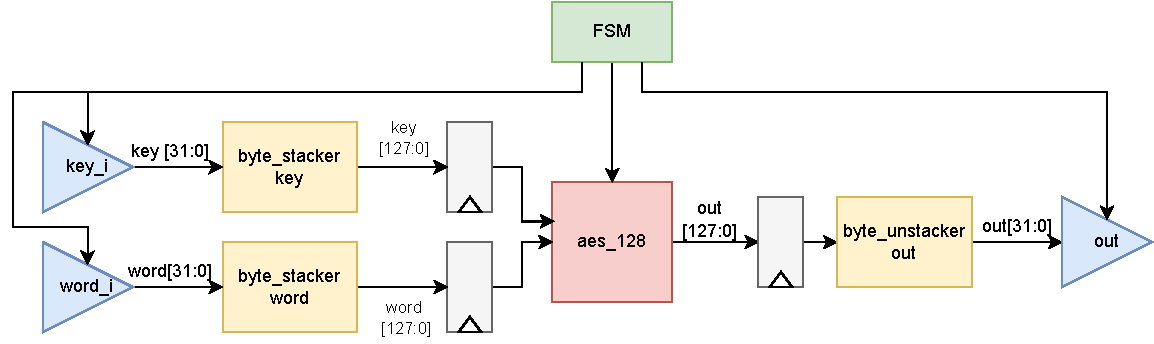
\includegraphics[width=0.95\textwidth]{hwpe_aes.pdf}
	\label{hwpe-aes}
	\caption{Block diagram of the implemented AES HWPE}
\end{figure}

The resulting AES HWPE is depicted in \Cref{hwpe-aes}. The input and output streamers are controlled by the FSM in the control block which uses the registers written by the CPU beforehand. All data path units use a simple ready/valid handshake to allow both forward and backward dependencies, e.g. if the AES unit is busy of no new data is provided by the input streamers yet. The registers were used to balance the pipeline, however no timing analysis has been undertaken to examine whether they are necessary eventually.

Additionally, a simple demo application comparable to the reference software demo was implemented. It writes input word and keys to the memory ($N$ times), sets all required control registers via the HWPE driver, and triggers $N$ encryptions. In the end, the results are again compared to their expected values.

\section{Results} \label{sec:results}

The key results achieved are summarised in \Cref{tab:results}. Clearly, the hardware implementation outperforms the software implementation in terms of runtime. Also the code size is notably reduced (most of the code size comes from the runtime code). The speed-up is likely do directly translate into energy savings as the CPU can enter a sleep mode after encryption more quickly. Unfortunately, issues with the synthesis scripting prevented area estimations. Still, the \verb|aes_128| IP core is very small (s. \Cref{tab:aes_cores}), thus the area overhead relative to the PULPissimo SoC should be minimal.

\begin{table}[h]
    \centering
    \begin{tabular}{c|c c}
        \toprule
         &  AES Software & AES HWPE  \\
        \midrule
		Runtime $N=32$ & \SI{2876}{\mu s} & \SI{10}{\mu s} \\
		Relative speed-up & 1 & 287.6 \\
		Runtime further encryption & \SI{61}{\mu s} & \SI{280}{ns} \\
		Code size & 9816 bytes & 9140 bytes\\
        \bottomrule
    \end{tabular}
	\label{tab:results}
	\caption{Simulation results for both AES implementations. The simulation clock frequency is \SI{50}{MHz} and the used engine was Mentor Questasim.}
\end{table}

\section{Summary and Outlook} \label{sec:summary}

During this project, a PULP hardware processing engine implementing AES encryption was designed and integrated into the PULPissimo SoC. As a result, an encryption speed-up of 287.6 was reached while decreasing the code size. However, this projects motivates further work. It might be interesting to support also more complex (but in reality inevitable) encryption modes like CBC. Furthermore it might be interesting to use modern lightweight cryptographic algorithms designed specifically for edge devices.

Besides that, an ASIC implementation of the AES HWPE could bring deeper insights into both area and power consumption. This also matches the PULPissimo philosophy which is using FPGA only as prototyping platform and is intended to be implemented as IC.

\clearpage
\sloppy
\printbibliography

\end{document}
